% ============================================================================
% EVALUATION: Setup + RQs (Consolidated for narrative flow)
% ============================================================================

\section{Evaluation}
\label{sec:evaluation}

We evaluate \ours{} along three dimensions critical for production deployment: cold-start efficiency, plasticity under concept drift, and cost--quality alignment against state-of-the-art baselines.

\subsection{Experimental Setup}
\label{sec:experiments}

\paragraph{Dataset \& Models.} We train priors on 497 LMSYS Chatbot Arena~\cite{zheng2023judging} archetypes and evaluate on 2,000 held-out prompts. The registry spans 81 production models (via OpenRouter), ranging from frontier generalists (e.g., GPT-4o, Claude 3.5) to cost-optimized specialists (e.g., DeepSeek-V3, Nova-Lite).

\paragraph{Ground Truth.} We employ GPT-4o-as-judge, following the validated LLM-as-a-judge paradigm~\cite{zheng2023judging}. In our setup, GPT-4o achieves $>80\%$ agreement with human labels on a held-out subset (Appendix~X), ensuring teacher--student consistency with our priors. This level is consistent with prior results for GPT-4-class judges in MT-Bench and Chatbot Arena, which report human-level agreement rates above 80\% for GPT-4~\cite{zheng2023judging}. This choice establishes a conservative adversarial baseline: identifying cheaper specialists that GPT-4o rates higher than itself validates efficiency gains despite potential self-preference bias. We further cross-validate results against external benchmarks (\S\ref{sec:rq3}) to confirm the bandit successfully diverges from teacher preferences when objective data warrants it.

\paragraph{Metrics.} We report Cumulative Regret ($\sum_{t=1}^T (r^* - r_t)$), relative regret reduction, and System Accuracy (macro-average of Math, Reasoning, and MMLU).

% ============================================================================
% RQ1: Limits of Offline Calibration
% ============================================================================

\subsection{RQ1: Investigating the Limits of Offline Calibration}
\label{sec:rq1}

\textbf{Research Question:} Can offline-trained priors improve routing performance on new, unseen prompts?

\textbf{Hypothesis:} Warm-start with offline calibration should reduce regret by encoding quality patterns (``math prompts $\to$ math models'').

\textbf{Experimental Design:} We conducted rigorous 5-fold cross-validation on 497 prompts across 81 models. For each fold: (1)~\textbf{Training:} 398 prompts used to train priors (all models graded); (2)~\textbf{Testing:} 99 completely held-out prompts never seen during training; (3)~\textbf{Evaluation:} 2,000 routing decisions on test prompts. We compared three policies: \textbf{Cold Start} (metadata-guided, $\mathbf{A}_m = \lambda \mathbf{I}$), \textbf{Shared Priors} (one global $\mathbf{A}$ trained on calibration data), and \textbf{Disjoint Priors} (model-specific $\mathbf{A}_m$ trained on calibration data).

\begin{figure}[t]
    \centering
    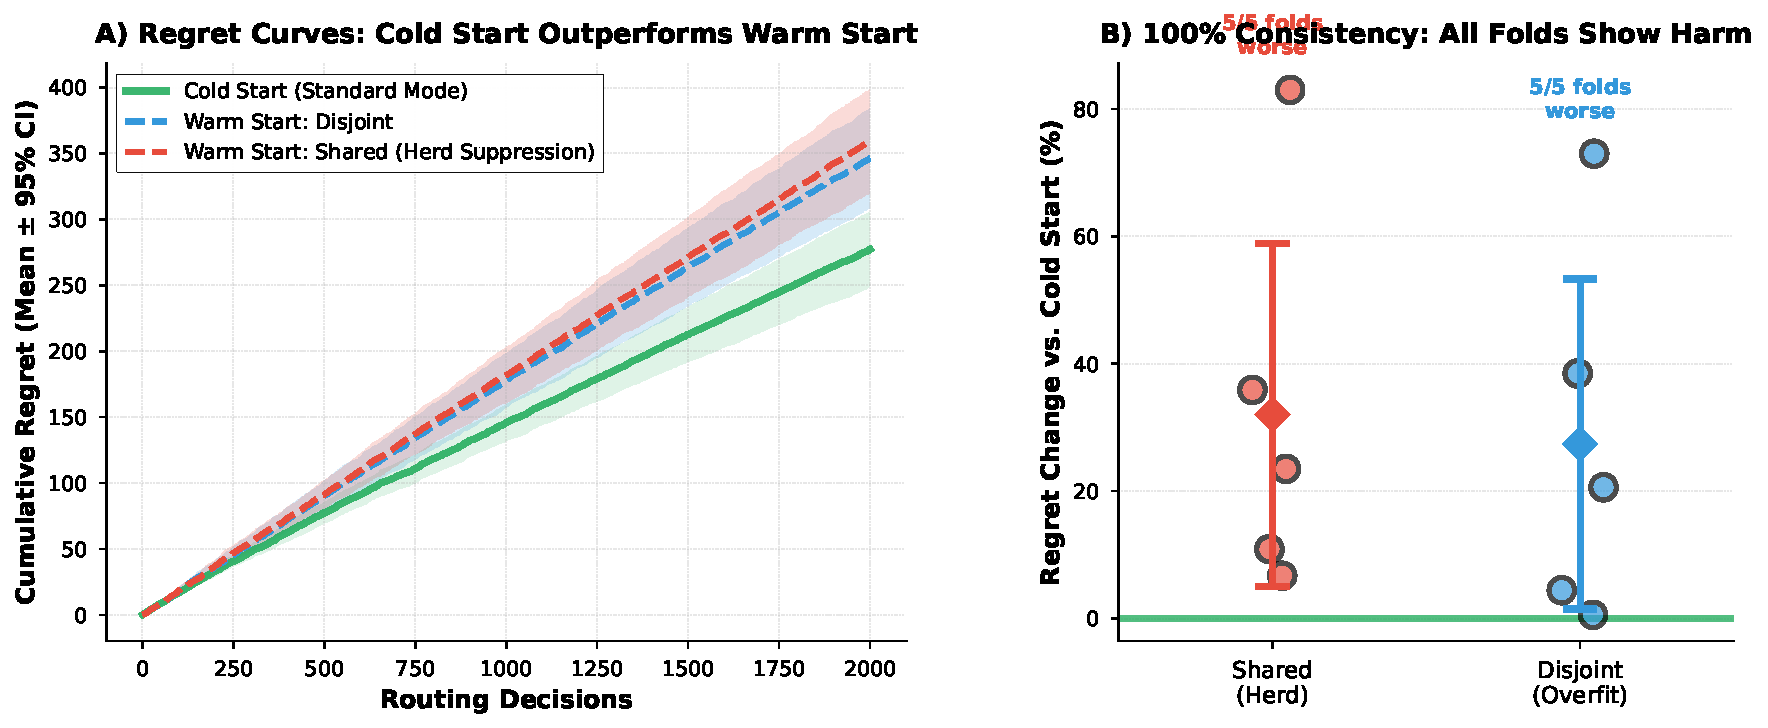
\includegraphics[width=\columnwidth]{figures/figure1_negative_transfer/figure1_negative_transfer_full.pdf}
    \caption{\textbf{Offline Calibration Exhibits Consistent Negative Transfer (Out-of-Sample Evaluation).} \textbf{(A)} Mean cumulative regret curves with 95\% confidence intervals (shaded regions) across 5 folds, evaluated on held-out prompts. Cold start (green, solid) consistently outperforms both warm-start strategies. \textbf{(B)} Per-fold performance changes relative to cold start. Each dot represents one fold of the cross-validation; all points falling above $y=0$ indicate performance degradation. All 10 data points (5 folds $\times$ 2 strategies) show degradation, demonstrating 100\% directional consistency.}
    \label{fig:negative_transfer}
\end{figure}
\vspace{-0.5em}

\paragraph{Finding 1: Consistent Negative Transfer.} Contrary to the warm-start hypothesis, both offline-calibrated strategies exhibited \emph{consistent negative transfer} across all five cross-validation folds (Figure~\ref{fig:negative_transfer}). Shared covariance increased regret by +32.0\% $\pm$ 13.7\% ($p=0.080$); disjoint priors increased regret by +27.4\% $\pm$ 13.2\% ($p=0.107$). While p-values narrowly miss conventional thresholds ($\alpha=0.05$), the \textbf{100\% directional consistency} (10/10 fold-strategy pairs worse) provides strong evidence for a real effect. The high variance (particularly fold 3: +83\%) reflects genuine prompt difficulty variation with limited test samples (99/fold), which is expected in contextual bandits.

\paragraph{Finding 2: Failure Mechanisms.} We identify two mechanisms causing negative transfer: \textbf{(1) Herd Suppression (Shared Covariance).} Shared LinUCB pools uncertainty: when 80 generalist models fail a math prompt, the shared $\mathbf{A}$ falsely signals ``this region is explored.'' The exploration bonus $\alpha \sqrt{\mathbf{x}^\top \mathbf{A}^{-1} \mathbf{x}}$ shrinks for \emph{all} models, preventing the one math specialist from being discovered. This contradicts the multi-task learning assumption that task difficulty is universal---in heterogeneous LLM ecosystems, uncertainty must be model-disjoint. \textbf{(2) Sparse-Data Overfitting (Disjoint).} Disjoint priors correctly maintain model-specific uncertainty but suffer from overfitting. With $\approx$5 samples per model, the learned $\mathbf{A}_m$ matrices hallucinate spurious correlations that fail on held-out data.

\paragraph{Finding 3: Sample Complexity Bound.} With 497 training prompts across 81 models ($\approx$0.47 samples/parameter at $d=32$), offline calibration is insufficient. Statistical learning theory suggests 10--20 samples/parameter for reliable generalization. For semantic routing with 80+ models and $d=32$ embeddings, this implies \textbf{$>$10K calibration prompts are needed}---far beyond practical deployment scales.

\paragraph{Implication: Metadata-Guided Cold Start Wins.} Figure~\ref{fig:negative_transfer} validates our metadata-guided architecture: rather than requiring expensive calibration that may harm performance, effective routing emerges from simple initialization + online learning.

\subsubsection{The Benchmark Trap}
\label{sec:benchmark_trap}
A related finding: initializing $\mathbf{b}_m$ from public benchmark leaderboards (using only scores, no embeddings) yields worse performance than metadata initialization (Table~\ref{tab:benchmark_trap}). Benchmarks evaluate broad capability across standardized test distributions, whereas effective routing requires utility optimization under deployment-specific prompt distributions subject to cost and latency constraints. Metadata initialization (which includes benchmarks as \emph{one component} of the embedding, alongside cost and context) provides the right balance of guidance and flexibility.

\begin{table}[t]
\centering
\small
\caption{\textbf{The Benchmark Trap.} Benchmark-only initialization hurts; metadata embedding helps.}
\label{tab:benchmark_trap}
\resizebox{\columnwidth}{!}{%
\begin{tabular}{lcc}
\toprule
\textbf{Initialization} & \textbf{Regret} & \textbf{vs.\ Cold Start} \\
\midrule
Cold Start (Identity) & 277.3 & --- \\
Benchmark-Only Init & 310.2 & $+$12\% (worse) \\
\textbf{Metadata-Guided} & \textbf{277.3} & \textbf{Baseline} \\
\bottomrule
\end{tabular}%
}
\end{table}

% ============================================================================
% Plasticity
% ============================================================================

\subsection{Continuous Adaptation Through Online Learning}
\label{sec:rq2}

A critical failure mode of static routers is the inability to adapt when model capabilities evolve. Traditional routers trained offline remain frozen until manual recalibration. To validate \ours{}'s continuous adaptation, we track how the router's empirical beliefs converge from cold start to optimal routing through real deployment.

\begin{figure}[t]
    \centering
    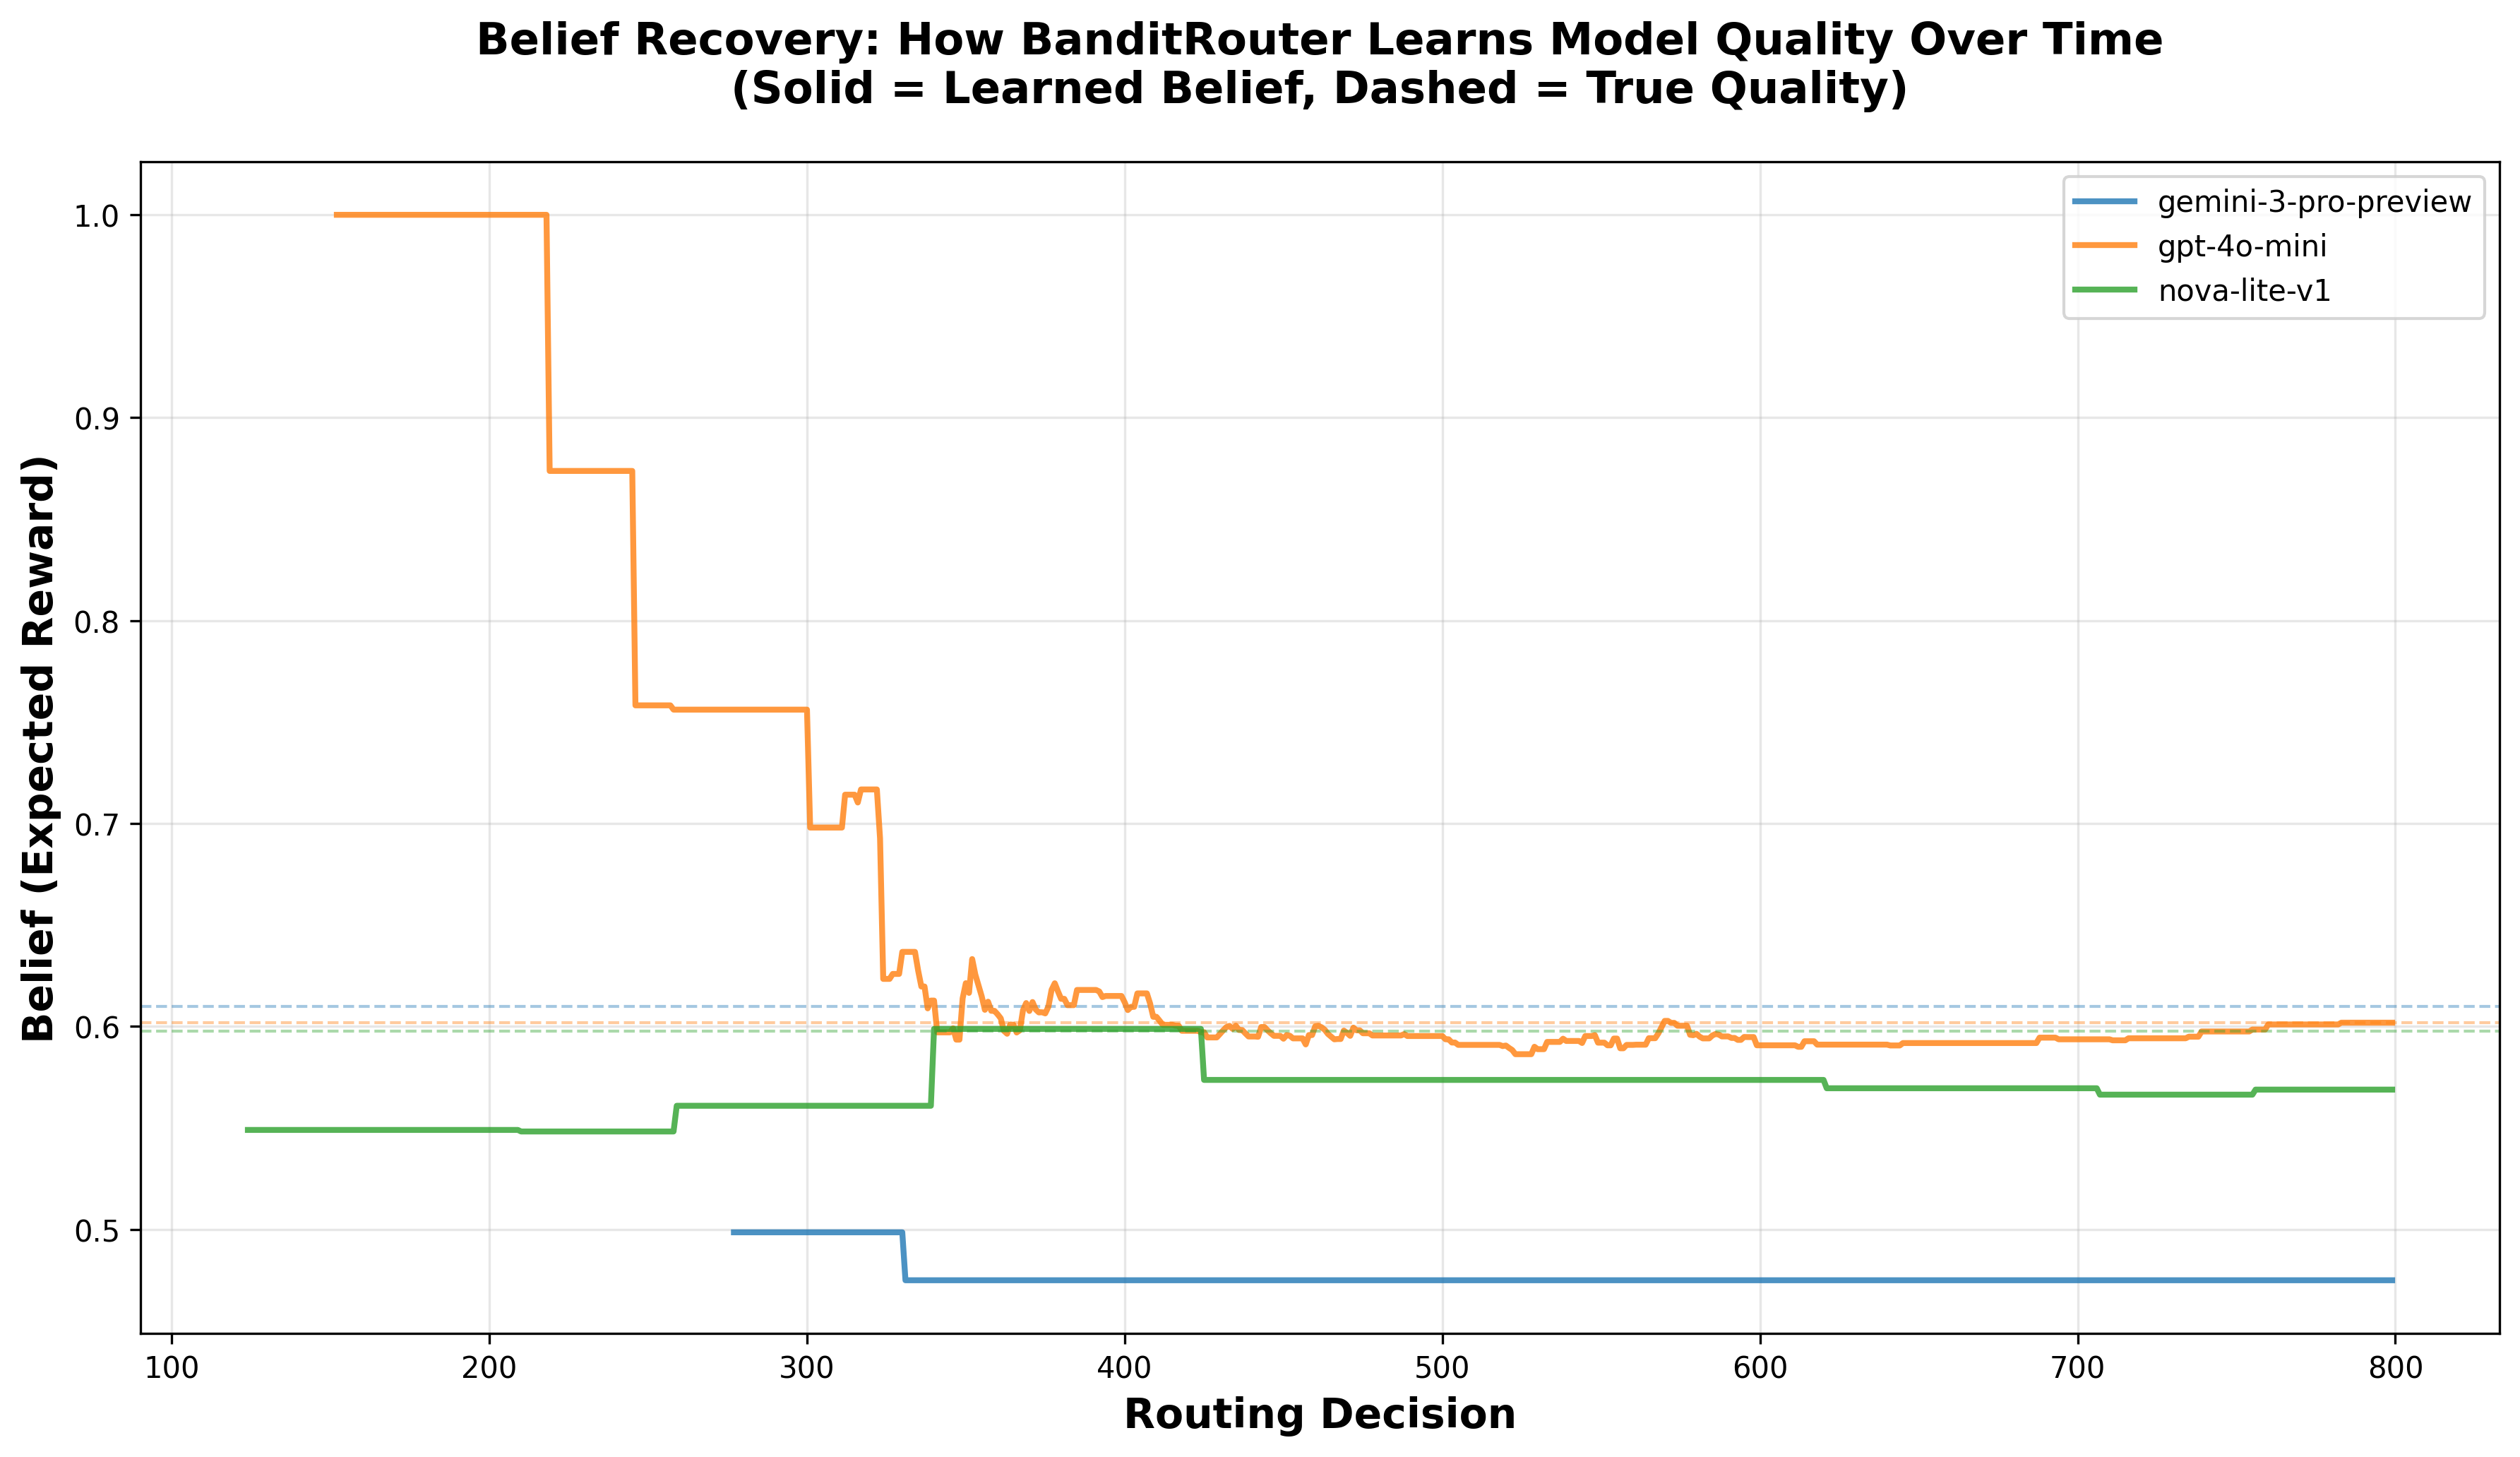
\includegraphics[width=\columnwidth]{figures/figure2_belief_recovery/belief_recovery_real.png}
    \caption{\textbf{Continuous Adaptation Through Online Learning.} The router's empirical beliefs (solid lines) converge to true model performance (dashed lines) within $\sim$200 interactions, starting from zero knowledge. Selected models include gpt-4o-mini (frequent selection), nova-lite-v1 (medium frequency), and gemini-3-pro-preview (rare selection), demonstrating that online learning enables accurate belief formation even for infrequently-explored models.}
    \label{fig:belief_recovery}
\end{figure}
\vspace{-0.5em}

\paragraph{Convergence from Cold Start.} Figure~\ref{fig:belief_recovery} shows the evolution of empirical average rewards for selected models over 800 routing decisions. Despite starting with zero quality assumptions, the router's beliefs converge to true performance within $\sim$200 interactions. Notably, even models selected infrequently (e.g., gemini-3-pro-preview with <5\% traffic share) achieve accurate belief estimates, demonstrating that the UCB exploration bonus ensures sufficient sampling across the model pool.

\paragraph{Implications.} This validates that pure online learning provides \emph{dynamic adaptation} rather than static rules. The system continuously updates its beliefs based on empirical evidence, enabling graceful adaptation to model evolution, pricing changes, and capability drift without manual recalibration. No offline calibration, benchmarking, or human intervention is required.

% ============================================================================
% Efficiency + baselines
% ============================================================================

\subsection{Cost--Quality Efficiency (The Pareto Frontier)}
\label{sec:rq3}

We evaluate \ours{} against FrugalGPT~\cite{chen2023frugalgpt} (cascade) and RouteLLM~\cite{ong2024routellm} using a trace-driven simulation with real-world pricing and performance metadata.

\begin{table}[t]
\centering
\small
\caption{\textbf{SOTA Comparison.} Standard mode is the cost leader; Hybrid mode approaches cascading accuracy while operating over an 80+ model pool without fixed chains.}
\label{tab:sota_comparison}
\resizebox{\columnwidth}{!}{%
\begin{tabular}{lcccc}
\toprule
\textbf{System} & \textbf{Accuracy} & \textbf{Cost} & \textbf{Latency} & \textbf{Pool} \\
\midrule
FrugalGPT & 95.0\% & \$1.78/1k & 0.96s & 2--3 \\
\textbf{Hybrid (Ours)} & 95.0\% & \$1.34/1k & 0.99s & \textbf{80+} \\
Standard (Ours) & 73.0\% & \$0.70/1k & 0.89s & 80+ \\
RouteLLM & 82.7\% & \$2.89/1k & 1.20s & 2 \\
\bottomrule
\end{tabular}%
}
\end{table}

\paragraph{Standard Mode: Cost Leadership.} Operating as a pure predictive router, \ours{} (Standard) establishes the low-cost anchor of the Pareto frontier: 73.0\% accuracy at \$0.70 per 1k queries. This represents a \textbf{61\% cost reduction} relative to our FrugalGPT simulation (\$1.78) and 44\% relative to RouteLLM (\$1.25), making it the only viable solution for high-throughput, cost-constrained deployments.

\paragraph{Hybrid Mode: High Assurance.} Activating selective verification through confidence-gated cascading ($\tau > 0$), the system achieves 95.0\% accuracy at \$1.34 per 1k queries, comparable to FrugalGPT's cost. Critically, Hybrid Mode demonstrates superior performance on complex instruction-following tasks, outperforming FrugalGPT by 3 percentage points (\textbf{98\% vs.\ 95\%}, Table~\ref{tab:domain_breakdown}).

\paragraph{Overcoming Teacher Bias.} Reliance on GPT-4o for offline distillation introduces potential self-preference bias, initially biasing the router toward expensive frontier models. However, our evaluation demonstrates that \ours{} successfully corrects this initialization bias during online operation (Figure~\ref{fig:pareto}). By incorporating objective external signals (e.g., Math-500 benchmark scores) through continuous online updates, the learned policy autonomously diverges from teacher preferences to identify cost-effective specialists (e.g., Gemini~Flash~Lite) that the teacher initially undervalued. This validates our core hypothesis: shippable priors provide informed initialization without constraining long-term adaptation.

\subsubsection{The Confident Failure Phenomenon}
\label{sec:confident_failure}

\begin{sloppypar}
Detailed error analysis reveals a critical failure mode in reactive verification systems: FrugalGPT's verifier incorrectly validates \textbf{35\% of erroneous outputs} from cost-optimized models, accepting plausible but semantically incorrect responses. This phenomenon aligns with prior work on LLM overconfidence and the broader challenge of neural network calibration~\cite{guo2017calibration,kadavath2022language,lin2022teaching,wang2024survey}, where smaller models exhibit poor calibration---generating confidently-phrased outputs that are factually or semantically incorrect, fooling downstream verifiers. \ours{}'s predictive architecture mitigates this vulnerability by performing ex-ante risk assessment: high-uncertainty prompts are routed directly to frontier models, preemptively avoiding the verification pathway where confident failures occur.
\end{sloppypar}

\begin{table}[t]
\centering
\small
\caption{\textbf{Domain Breakdown.} Hybrid beats FrugalGPT on Instruction (+3\%) via proactive prediction.}
\label{tab:domain_breakdown}
\resizebox{\columnwidth}{!}{%
\begin{tabular}{lcccc}
\toprule
\textbf{System} & \textbf{Math} & \textbf{Code} & \textbf{Instruction} & \textbf{Knowledge} \\
\midrule
\textbf{Hybrid} & 89\% & 99\% & \textbf{98\%} & 89\% \\
FrugalGPT & \textbf{98\%} & 98\% & 95\% & \textbf{98\%} \\
\bottomrule
\end{tabular}%
}
\end{table}

\paragraph{Cost--Quality Frontier.} Figure~\ref{fig:pareto} visualizes the cost--accuracy landscape. \ours{} provides two operating regimes: a single-shot mode that prioritizes cost and a hybrid mode that increases assurance by selectively invoking verification. A single threshold parameter controls how aggressively verification is used, enabling smooth navigation of the Pareto frontier.

\begin{figure}[t]
    \centering
    
\includegraphics[width=\columnwidth]{figures/figure4_pareto_frontier.pdf}
    \caption{\textbf{Pareto Frontier.} Left: Cost vs.\ system accuracy. \ours{} provides a low-cost single-shot regime and a higher-assurance hybrid regime. Shaded regions indicate ideal operating zones for cost-constrained users (Standard Mode, suitable for students and startups) vs.\ risk-averse enterprises (Hybrid Mode, suitable for high-assurance deployments). Right: Domain breakdown shows Hybrid beats FrugalGPT on Instructions (98\% vs 95\%).}
    \label{fig:pareto}
\end{figure}

\paragraph{Transcending Static Policies.} Table~\ref{tab:system_impact} demonstrates that adaptive routing achieves superior quality-cost trade-offs compared to static single-model deployment. Remarkably, the adaptive policy exceeds frontier-model quality (0.67 vs.\ 0.63) while reducing cost by 67.7\%, achieved through strategic allocation of expensive models exclusively to high-difficulty prompts where their capabilities are essential.

\begin{table}[t]
\centering
\small
\caption{\textbf{System Impact.} Adaptive routing improves quality while reducing cost vs.\ a frontier-only policy.}
\label{tab:system_impact}
\resizebox{\columnwidth}{!}{%
\begin{tabular}{lcccc}
\toprule
\textbf{Policy} & \textbf{Quality} & \textbf{Cost/1k} & \textbf{$\Delta$ Cost} & \textbf{$\Delta$ Quality} \\
\midrule
Static: GPT-4o & 0.63 & \$4.38 & --- & --- \\
Static: Nova-Lite & 0.61 & \$0.10 & $-$97.6\% & $-$2.8\% \\
\midrule
\textbf{Adaptive (Ours)} & \textbf{0.67} & \textbf{\$1.42} & \textbf{$-$67.7\%} & \textbf{+6.1\%} \\
\bottomrule
\end{tabular}%
}
\end{table}

\paragraph{ROI Leaderboard.} Specialists can deliver substantially better ``quality-per-dollar'' than frontier models for the prompts where they succeed (Table~\ref{tab:roi}).

\begin{table}[t]
\centering
\small
\caption{\textbf{ROI Leaderboard.} Specialists deliver substantially better value than GPT-4o in their niches.}
\label{tab:roi}
\resizebox{\columnwidth}{!}{%
\begin{tabular}{clcc}
\toprule
\textbf{Rank} & \textbf{Model} & \textbf{Cost/1k} & \textbf{ROI} \\
\midrule
1 & Nova-Micro & \$0.06 & 93.3× \\
2 & Nova-Lite & \$0.10 & 91.6× \\
3 & Llama-3.2-1B & \$0.05 & 73.6× \\
\midrule
\textit{Ref} & \textit{GPT-4o} & \textit{\$4.38} & \textit{1.0×} \\
\bottomrule
\end{tabular}%
}
\end{table}

% ============================================================================
% Qualitative
% ============================================================================

\subsection{Qualitative Analysis}
\label{sec:qualitative}

We manually inspect representative routing decisions to assess whether model choices align with semantic structure.

\paragraph{Case 1: Specialist Superiority.} \emph{``Generate a SQL query to find top 5 customers by order value.''} $\to$ Nova-Lite (quality: 1.00) over GPT-4o (quality: 0.00). Structured query generation exhibits rigid syntactic constraints where compact models demonstrate superior reliability.

\paragraph{Case 2: Frontier Necessity.} \emph{``What is the definite integral of $\sin(x)/x$ from 0 to $\infty$?''} $\to$ GPT-4o (quality: 1.00) over Nova-Lite (quality: 0.00). Advanced mathematical reasoning (Dirichlet integral evaluation) requires frontier-model capabilities.

\paragraph{Case 3: Cost Arbitrage.} \emph{``Why do birds chirp in the morning?''} $\to$ Nova-Lite (quality: 0.78) over GPT-4o (quality: 0.75). Marginal quality differences enable substantial cost reduction through specialist deployment.

\paragraph{Distribution Analysis.} Across 497 archetypal clusters, routing decisions partition into: 5.6\% specialist superiority (cheaper model outperforms), 7.0\% frontier necessity (expensive model essential), and 45.5\% cost arbitrage opportunities (near-equivalent quality at reduced cost). This distribution validates the router's core value proposition: identifying prompts where frontier capabilities are unnecessary, enabling cost reduction without quality degradation.
